\documentclass[onecolumn, draftclsnofoot,10pt, compsoc]{IEEEtran}
\usepackage{graphicx}
\usepackage{url}
\usepackage{setspace}
\usepackage{float}

\usepackage{geometry}
\geometry{textheight=9.5in, textwidth=7in}

% 1. Fill in these details
\def \CapstoneTeamName{Education Simulations}
\def \CapstoneTeamNumber{53}
\def \GroupMemberOne{Cameron Friel}
\def \GroupMemberTwo{Kelli Ann Ulep}
\def \GroupMemberThree{Samuel Wilson}
\def \CapstoneProjectName{Interactive 2D Simulations to Support Inquiry-Based Learning in Mechanical Engineering}
\def \CapstoneSponsorCompany{Oregon State University, School of Chemical, Biological, and Environmental Engineering}
\def \CapstoneSponsorPersonOne{Milo Koretsky}
\def \CapstoneSponsorPersonTwo{Tom Ekstedt}


% 2. Uncomment the appropriate line below so that the document type works
\def \DocType{		%Problem Statement
				%Requirements Document
				%Technology Review
				%Design Document
				Progress Report
				}
			
\newcommand{\NameSigPair}[1]{\par
\makebox[2.75in][r]{#1} \hfil 	\makebox[3.25in]{\makebox[2.25in]{\hrulefill} \hfill		\makebox[.75in]{\hrulefill}}
\par\vspace{-12pt} \textit{\tiny\noindent
\makebox[2.75in]{} \hfil		\makebox[3.25in]{\makebox[2.25in][r]{Signature} \hfill	\makebox[.75in][r]{Date}}}}
% 3. If the document is not to be signed, uncomment the RENEWcommand below
\renewcommand{\NameSigPair}[1]{#1}

%%%%%%%%%%%%%%%%%%%%%%%%%%%%%%%%%%%%%%%
\begin{document}
\begin{titlepage}
    \pagenumbering{gobble}
    \begin{singlespace}
    	
\includegraphics[height=4cm]{coe_v_spot1}
        \hfill 
        % 4. If you have a logo, use this includegraphics command to put it on the coversheet.
        %\includegraphics[height=4cm]{CompanyLogo}   
        \par\vspace{.2in}
        \centering
        \scshape{
            \huge CS Capstone \DocType \par
            {\large\today}\par
            \vspace{.5in}
            \textbf{\Huge\CapstoneProjectName}\par
            \vfill
            {\large Prepared for}\par
            \Huge \CapstoneSponsorCompany\par
            \vspace{5pt}
            {\Large
                \NameSigPair{\CapstoneSponsorPersonOne}\par
                \NameSigPair{\CapstoneSponsorPersonTwo}\par
            }
            {\large Prepared by }\par
            Group\CapstoneTeamNumber\par
            % 5. comment out the line below this one if you do not wish to name your team
            \CapstoneTeamName\par 
            \vspace{5pt}
            {\Large
                \NameSigPair{\GroupMemberOne}\par
                \NameSigPair{\GroupMemberTwo}\par
                \NameSigPair{\GroupMemberThree}\par
            }
            \vspace{20pt}
        }
        \begin{abstract}
         This document covers a brief overview of the purposes and goals of the Interact 2D Simulations to Support Inquiry-Based Learning in Mechanical Engineering project. It will then include sections covering the current progress that has been made in the project and the tasks that are still left to do before the beta due date. Following this is a section detailing any problems that have come up during the development process of the project. The final section in the document shows physical examples of the project in the form of images in order to view what the project looks like along with descriptions of what is going on within each image. 

        \end{abstract}     
    \end{singlespace}
\end{titlepage}
\newpage
\pagenumbering{arabic}
\tableofcontents
% 7. uncomment this (if applicable). Consider adding a page break.
%\listoffigures
%\listoftables
\clearpage

% briefly recap the project purposes and goals
% describe where you are currently on the project
% describe what you have left to do
% describe any problems that have impeded your progress, with any solutions you have
% include particularly interesting pieces of code (if coding is involved)
% (research only) include descriptions of preliminary results
% (interface design only) include description of first user study, hopefully with results
% include images of your project -- screen shots, photos, whatever is appropriate
% at least alpha level functionality should be in evidence at the draft turn-in (end of week 6), % with beta level functionality at the final submission (end of term).

\section{Purposes and Goals}
This project involves solving the problem of some universities lacking resources to visually show physical and mechanical interactions for Mechanical Engineering concepts in the classroom.
This project is built on the research that shows that students can achieve a better understanding of difficult concepts by learning through simulated environments that they can interact with. By implementing 2D simulations based on these concepts, students will be able to visually interpret the concepts in the course. We were tasked with creating six variations of a two dimensional simulation based on mechanical engineering concepts in order to support inquiry based learning for mechanical engineering students. The simulations will be handed over to the client at the end of the year to be hosted on the Concept Warehouse website, which is a website that provides interactive learning opportunities for classrooms. The goal for the simulations is to include real time mathematical feedback in the form of graphs and values within the simulation. There will also be buttons to start, stop, and reset the simulation, so a student can explore the simulation as many times or at as many points as they need to. The simulation will also allow  a student to be able to modify specific parameters within the simulation in the sixth variation of the simulation, such as mass, friction, and angles.

\section{Progress}
Currently, we have completed each of the five basic simulations for the project, as well as a fully functional exploratory mode. Each simulation has the start, stop, and reset buttons working, as well as graphs being live updated while the simulation is running. Variables that are particularly interesting in the simulation are displayed and updated to the user in real time to the user. Since each case is slightly different from the one before, once the first simulation was complete we were able to simply change some attributes or add another pendulum to get the rest of the simulations working. \newline
\noindent 
For the first simulation, we have developed a world where one pendulum rests at a 60 degree angle and swings to the other side. The start, pause, and reset buttons are present to allow the user to interact with the scene. There are also two values that are updated as the scene plays which include the simulation time and the height of the pendulum. There is a graph present which graphs the simulation time on the x-axis and the height of the pendulum on the y-axis. 

\begin{figure}[H]
  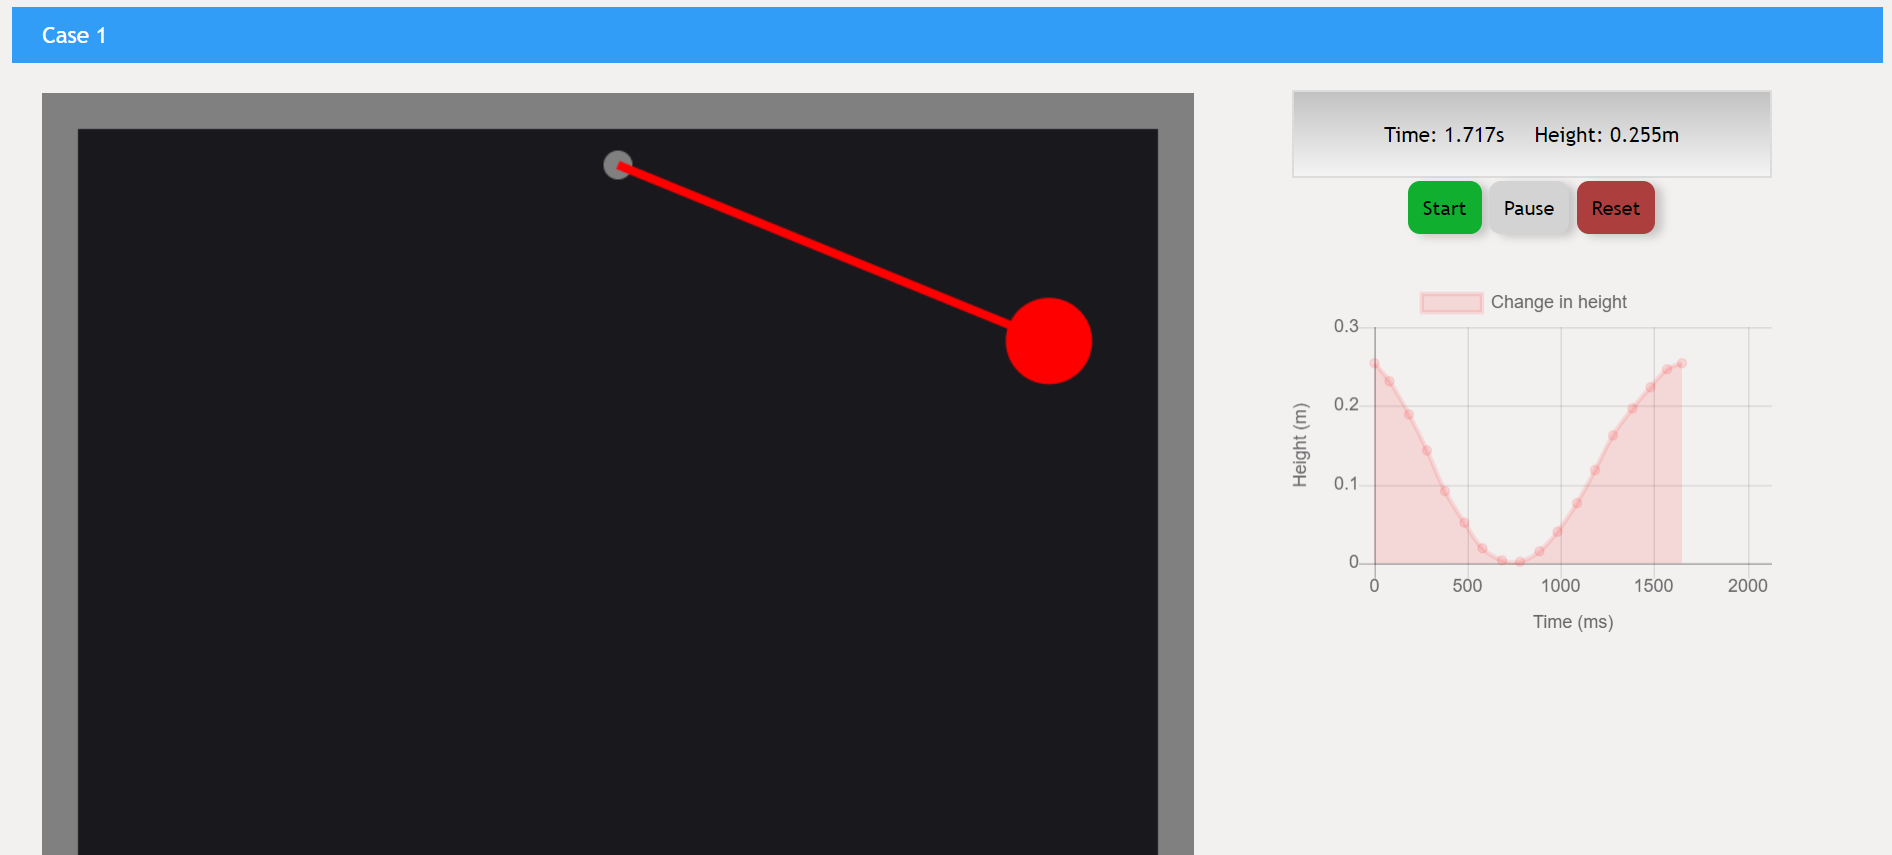
\includegraphics[width=5.5 in]{pictures_beta/case1_end.png}
  \caption{Case 1 - state after simulation ends }
  \label{fig:case1_end}
\end{figure}

\noindent 
The second simulation is similar to the first, however, instead of showing only one pendulum there are two present in the world with one resting at 60 degrees with a weight of 1.5 lbs while the other is resting at 0 degrees and has a weight of 1.5 lbs as well. The pendulum's weights have been set to a restitution of 0 in order to allow for a completely plastic collision, meaning that the weights stick together. To account for there being two pendulums, the live update table includes another height calculation for the second pendulum and is also graphed on the same chart as the first pendulum.


\begin{figure}[H]
  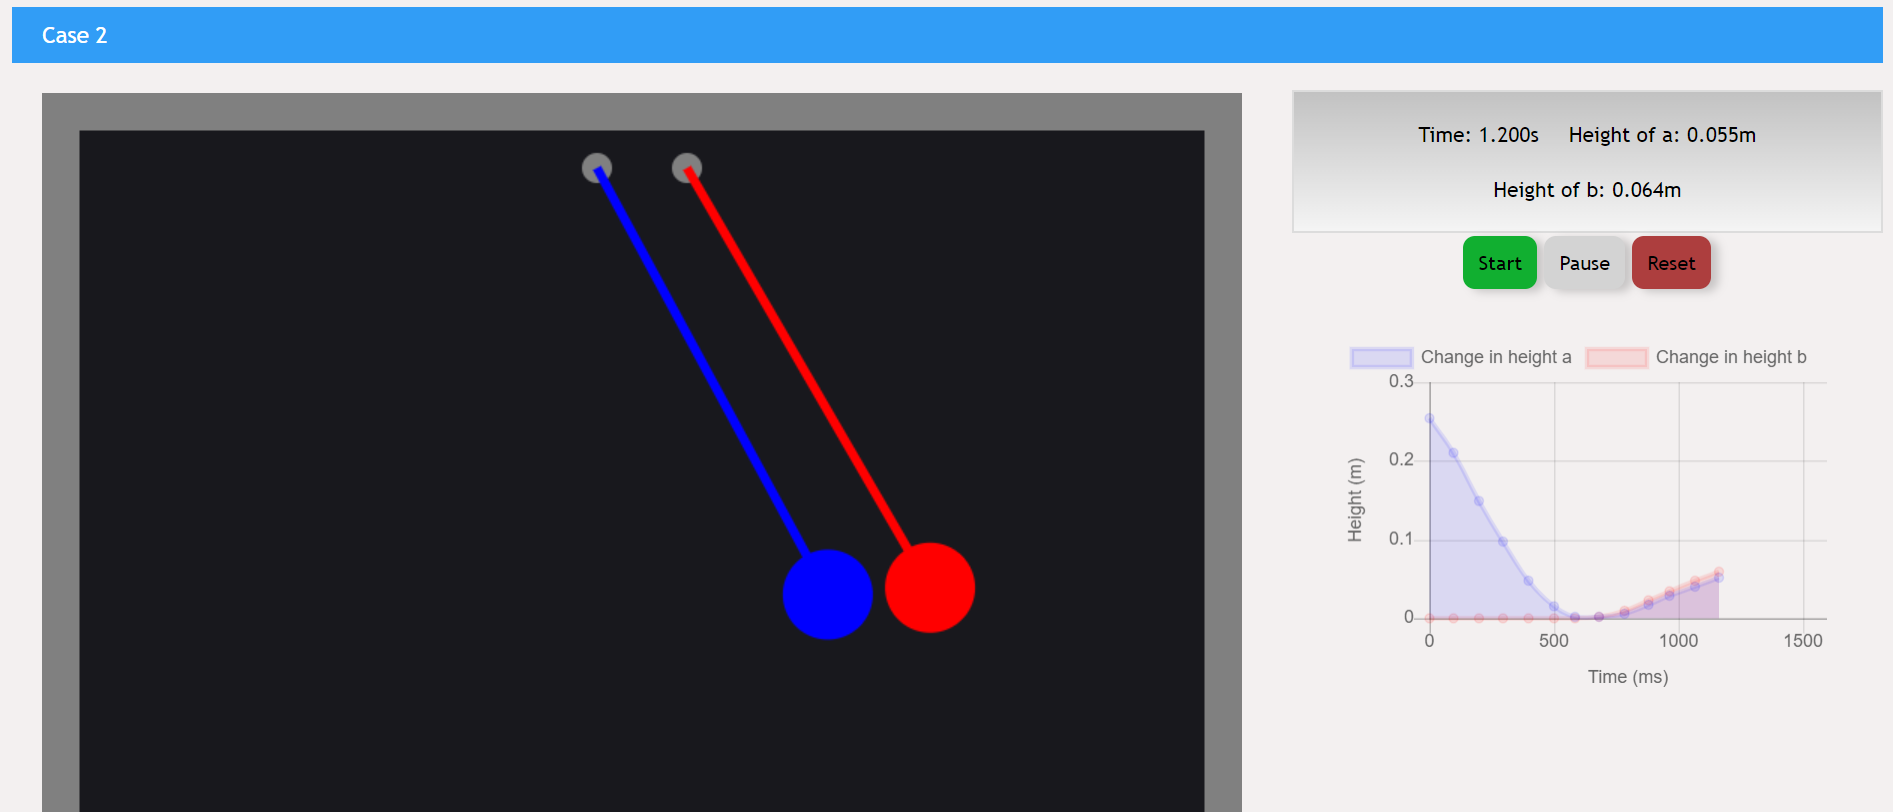
\includegraphics[width=5.5 in]{pictures_beta/case2_end.png}
  \caption{Case 2 - state after simulation ends }
  \label{fig:case2_end}
\end{figure}

\noindent 
The third simulation in set up the same as the previous simulation, however, the pendulum that is set to impact the resting pendulum at 0 degrees now has a weight of 3 lbs, 1.5 lbs greater than the pendulum it is impacting. 

\begin{figure}[H]
  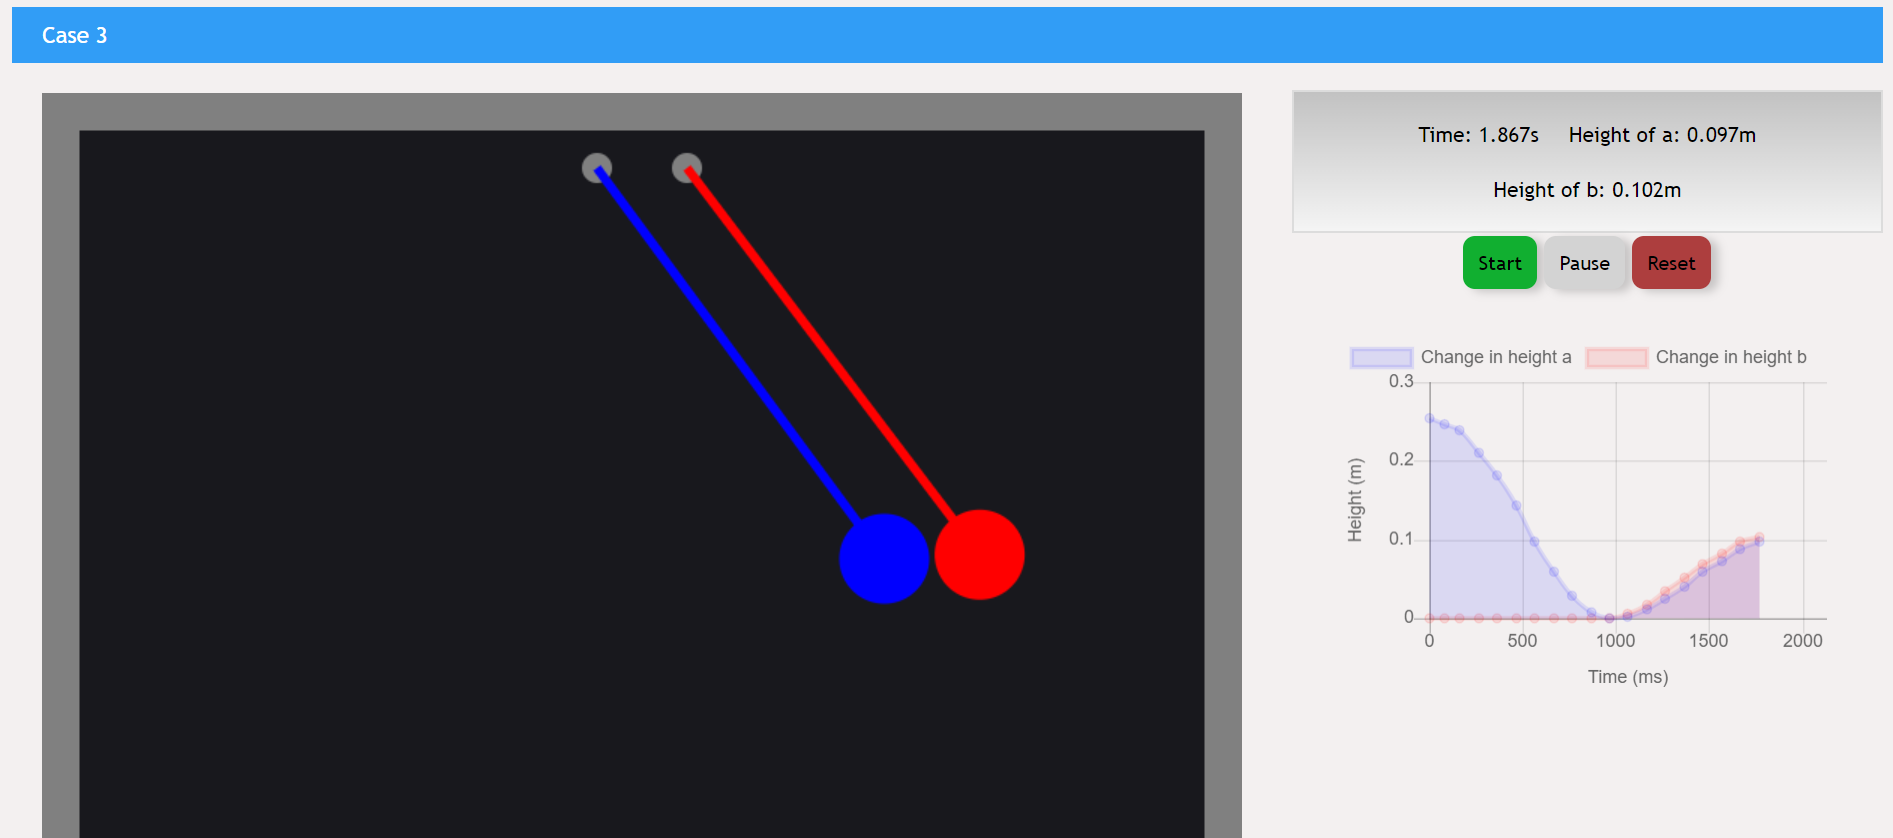
\includegraphics[width=5.5 in]{pictures_beta/case3_end.png}
  \caption{Case 3 - initial state }
  \label{fig:case3}
\end{figure}

\noindent 
The fourth simulation is set up to where both pendulums are at 1.5 lbs with a restitution set to 0 to allow for a completely plastic collision. The two pendulums are set up at -30 degrees and 30 degrees respectively. The live update table and graph is still present in this simulation. 

\begin{figure}[H]
  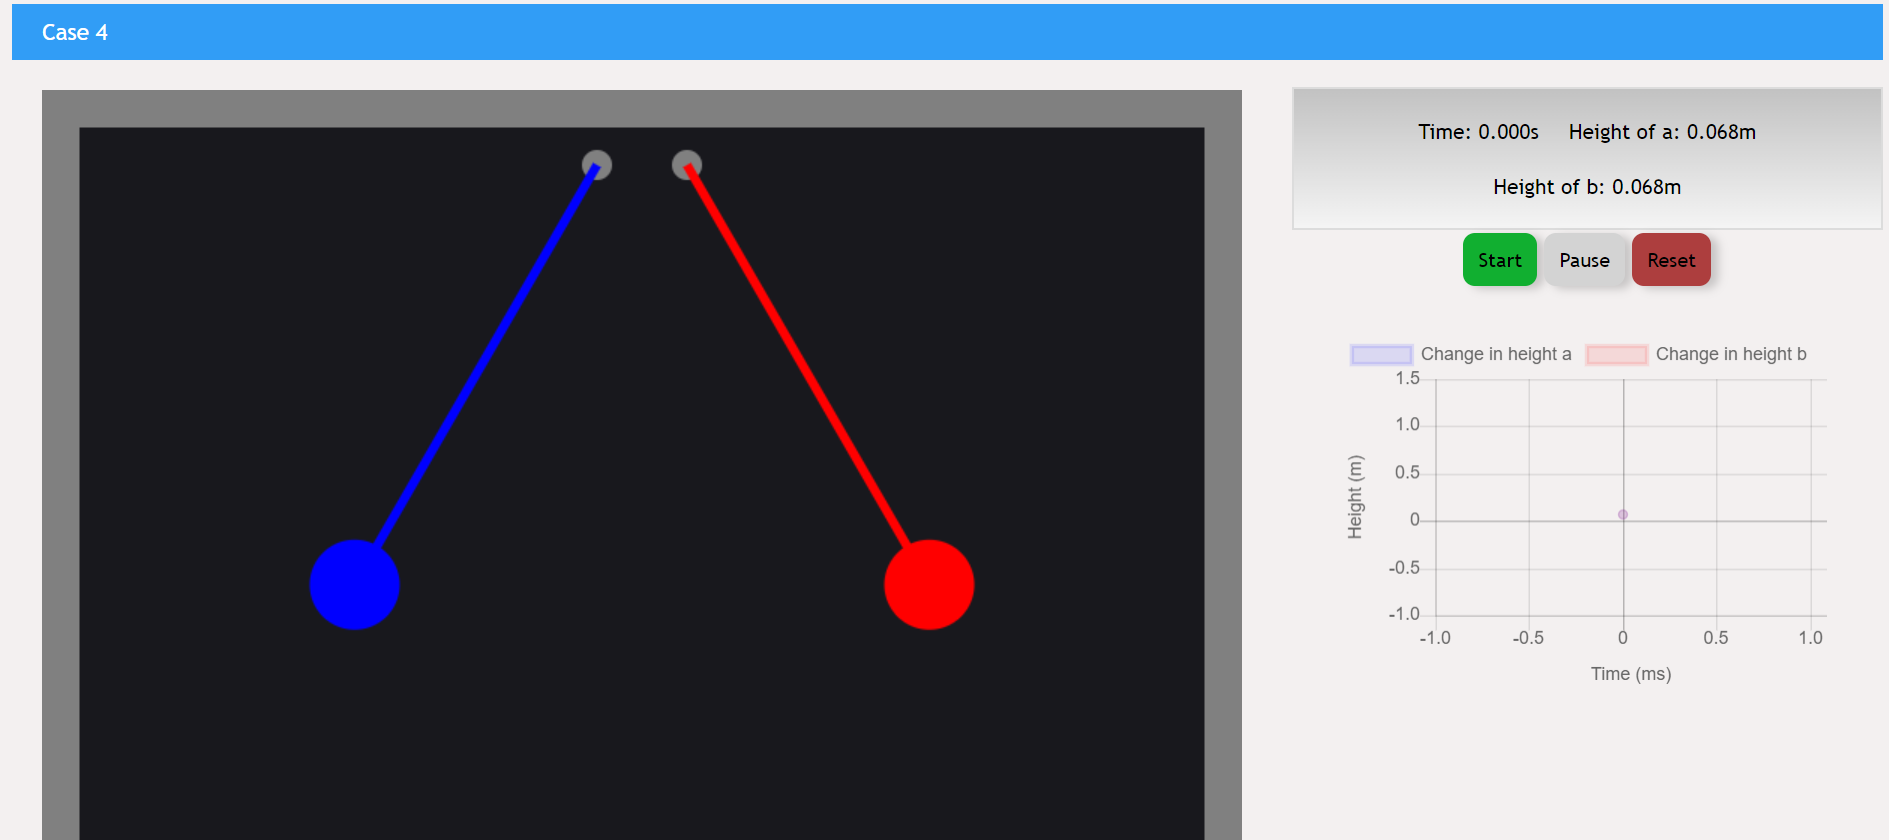
\includegraphics[width=5.5 in]{pictures_beta/case4_start.png}
  \caption{Case 4 - initial state }
  \label{fig:case4}
\end{figure}

\begin{figure}[H]
  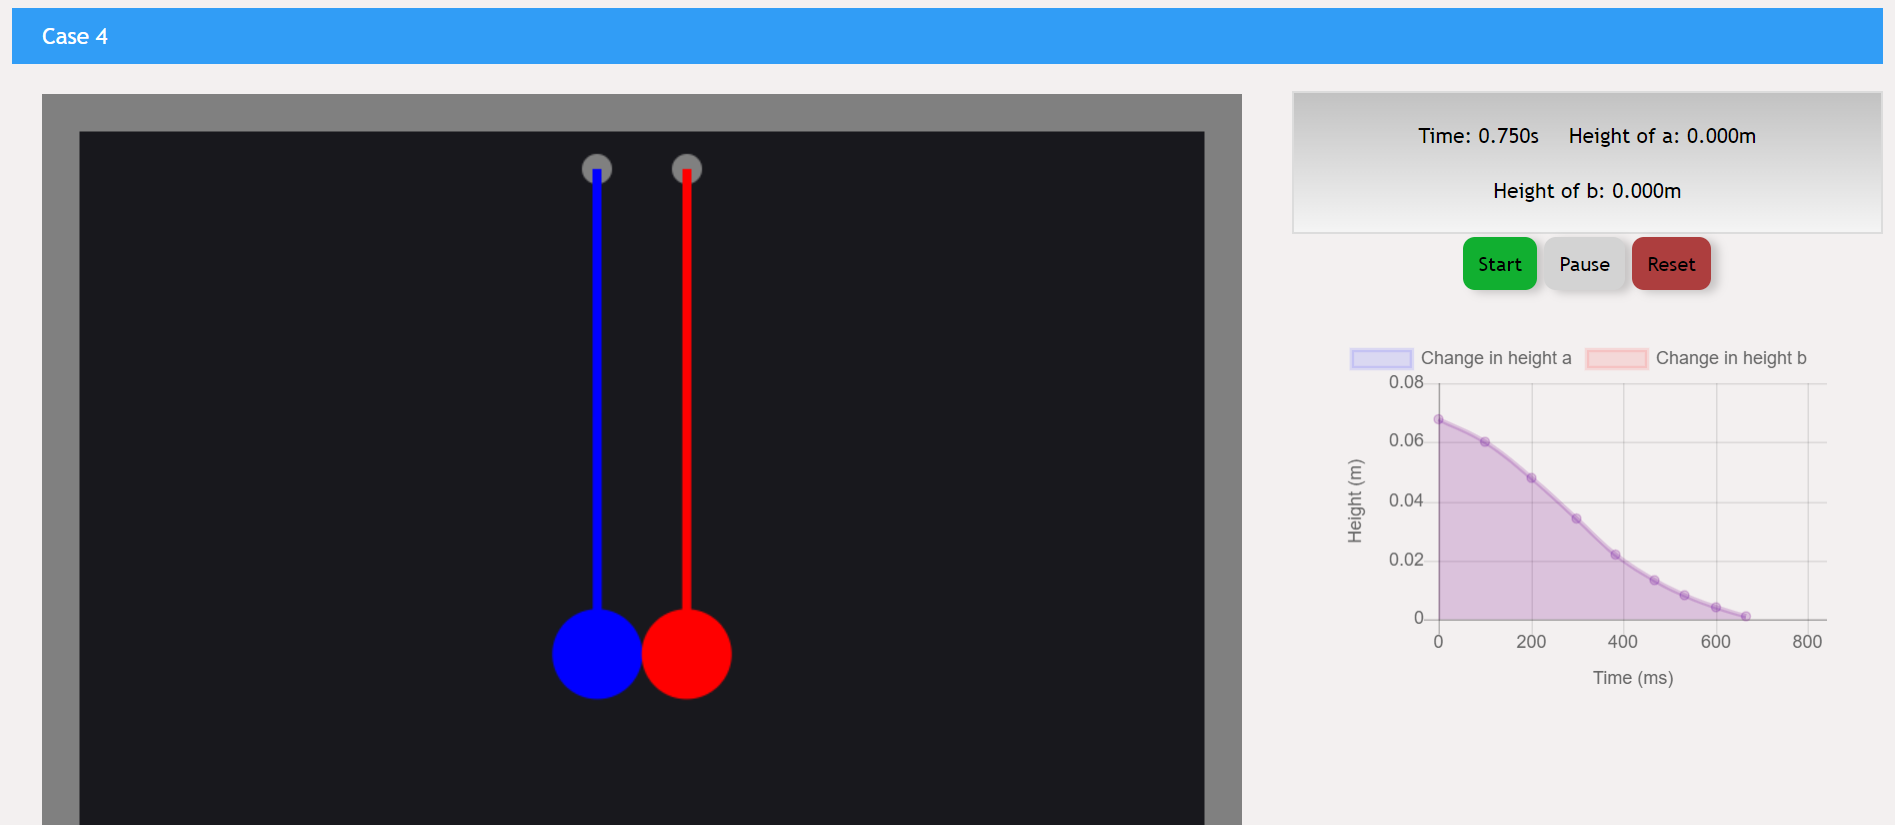
\includegraphics[width=5.5 in]{pictures_beta/case4_end.png}
  \caption{Case 4 - end state }
  \label{fig:case4}
\end{figure}

\noindent 
The fifth and final simulation is set up like the second simulation, however, the restitution is set to 1 so that the pendulums will have to bounce off of each other. 

\begin{figure}[H]
  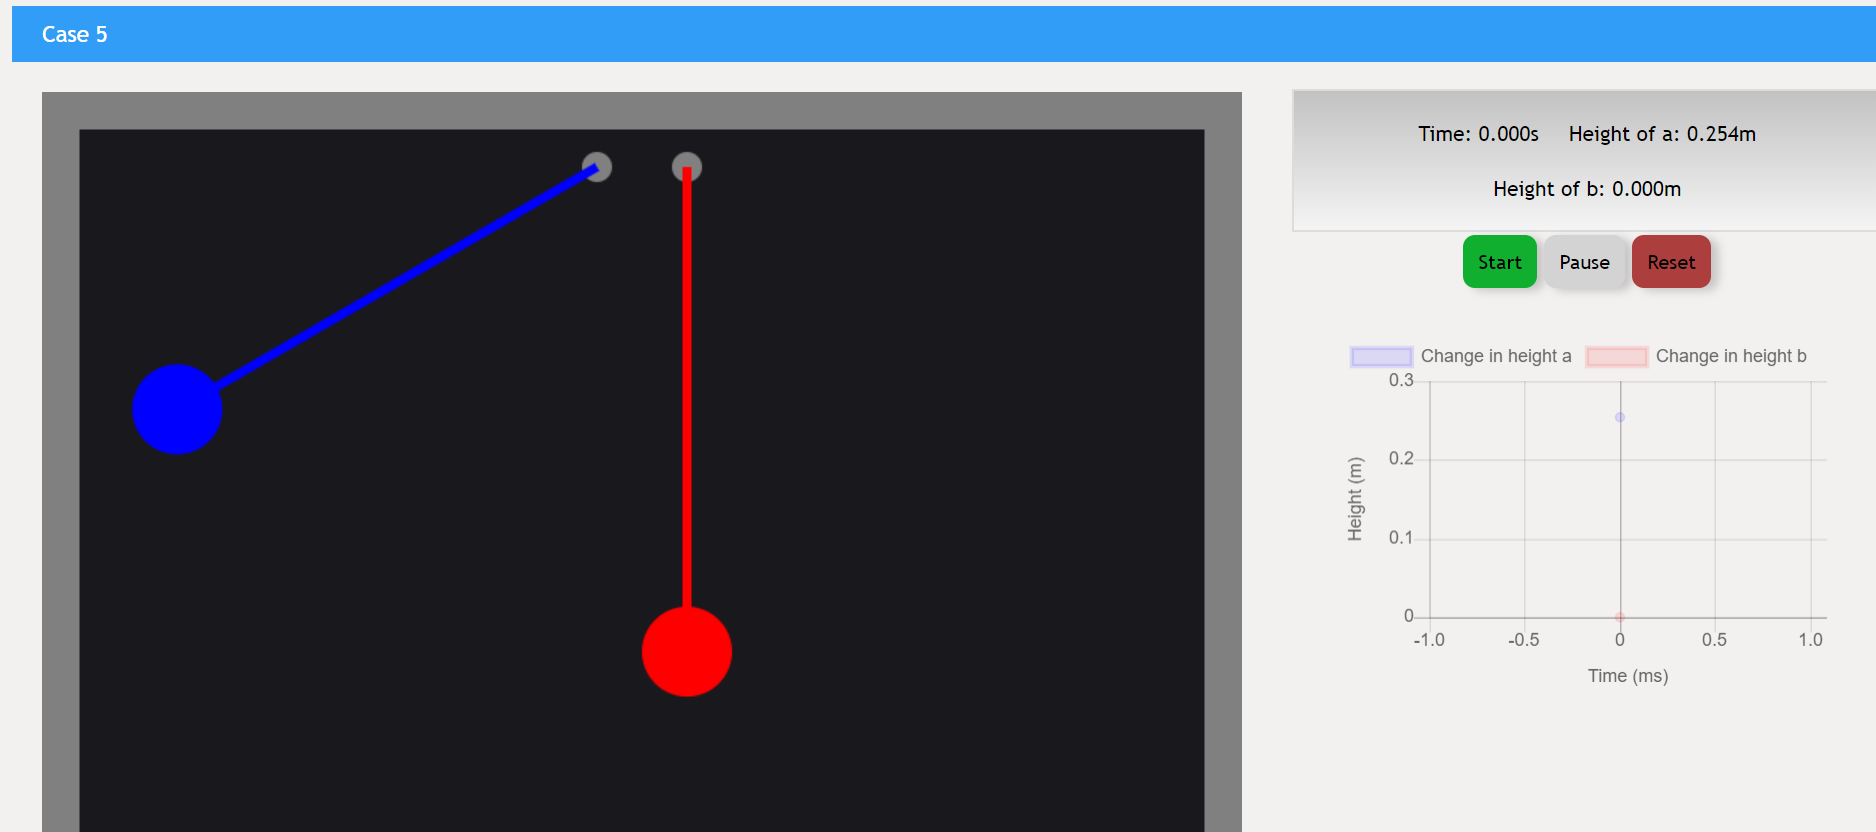
\includegraphics[width=5.5 in]{pictures_beta/case5_start.png}
  \caption{Case 5 - initial state }
  \label{fig:case5}
\end{figure}
\begin{figure}[H]
  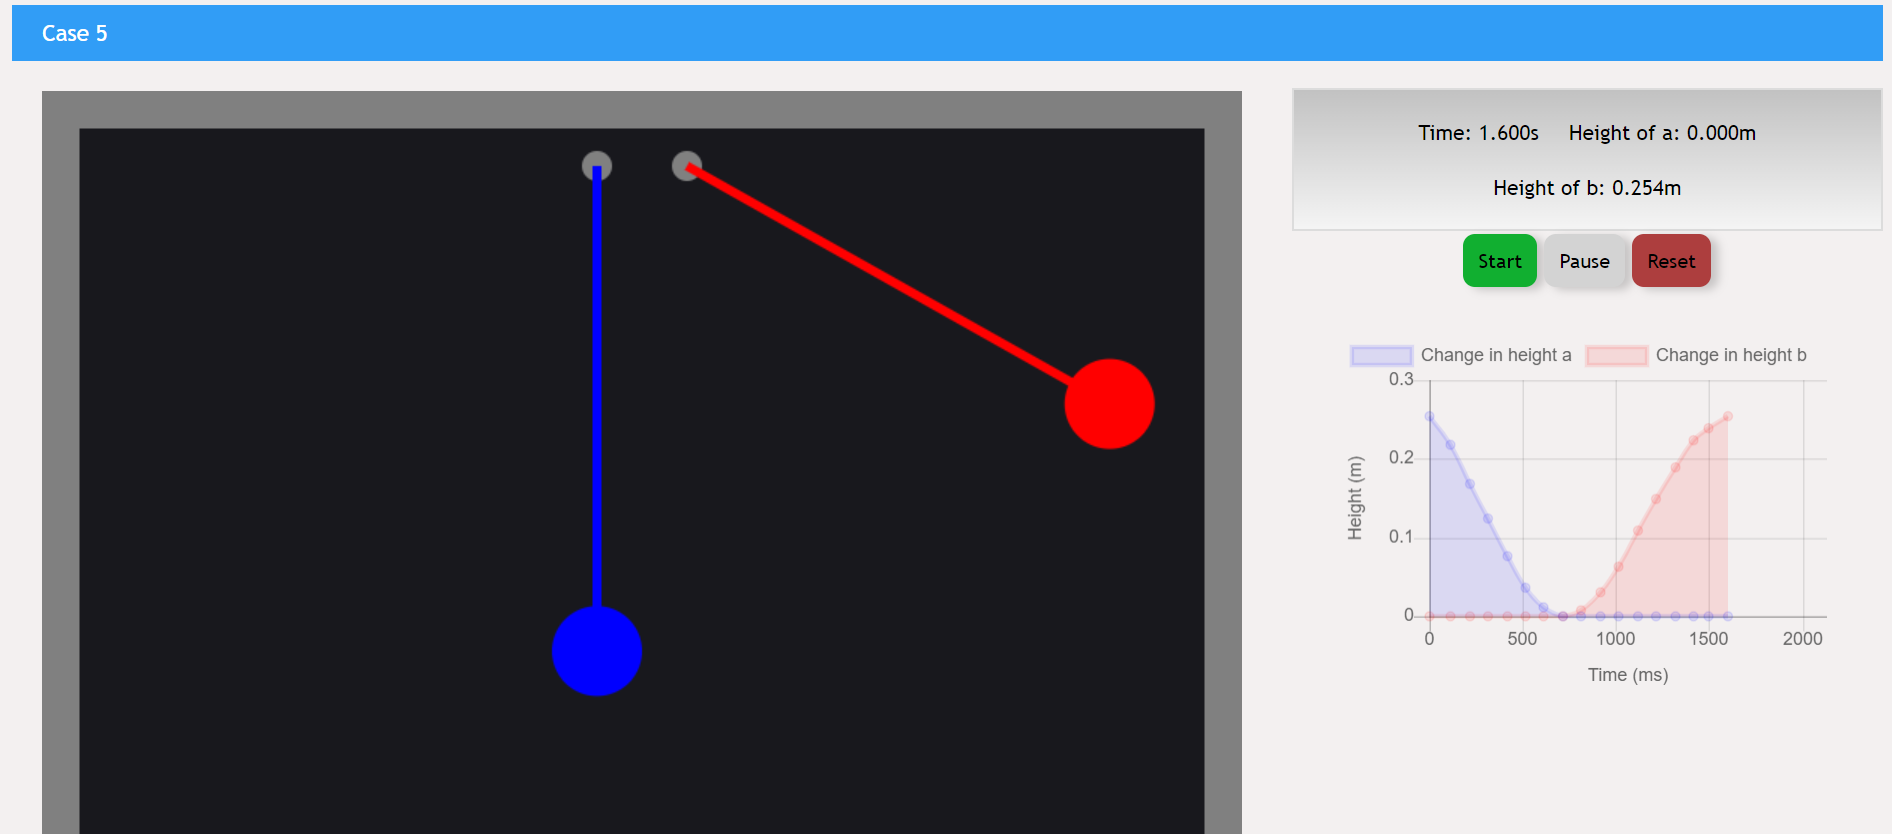
\includegraphics[width=5.5 in]{pictures_beta/case5_end.png}
  \caption{Case 5 - final state }
  \label{fig:case5}
\end{figure}

\noindent 
The exploratory mode was developed last and is a combination of each of the simulations that were created. It acts as a sandbox where the user can modify values within the world and observe the interactions that take place. There are sliders included on the page that modify a pendulum's mass, length, weight, and restitution. The user can also set if they want one or two pendulums. The same live update table is included along with the graph to observe the data. 

\begin{figure}[H]
  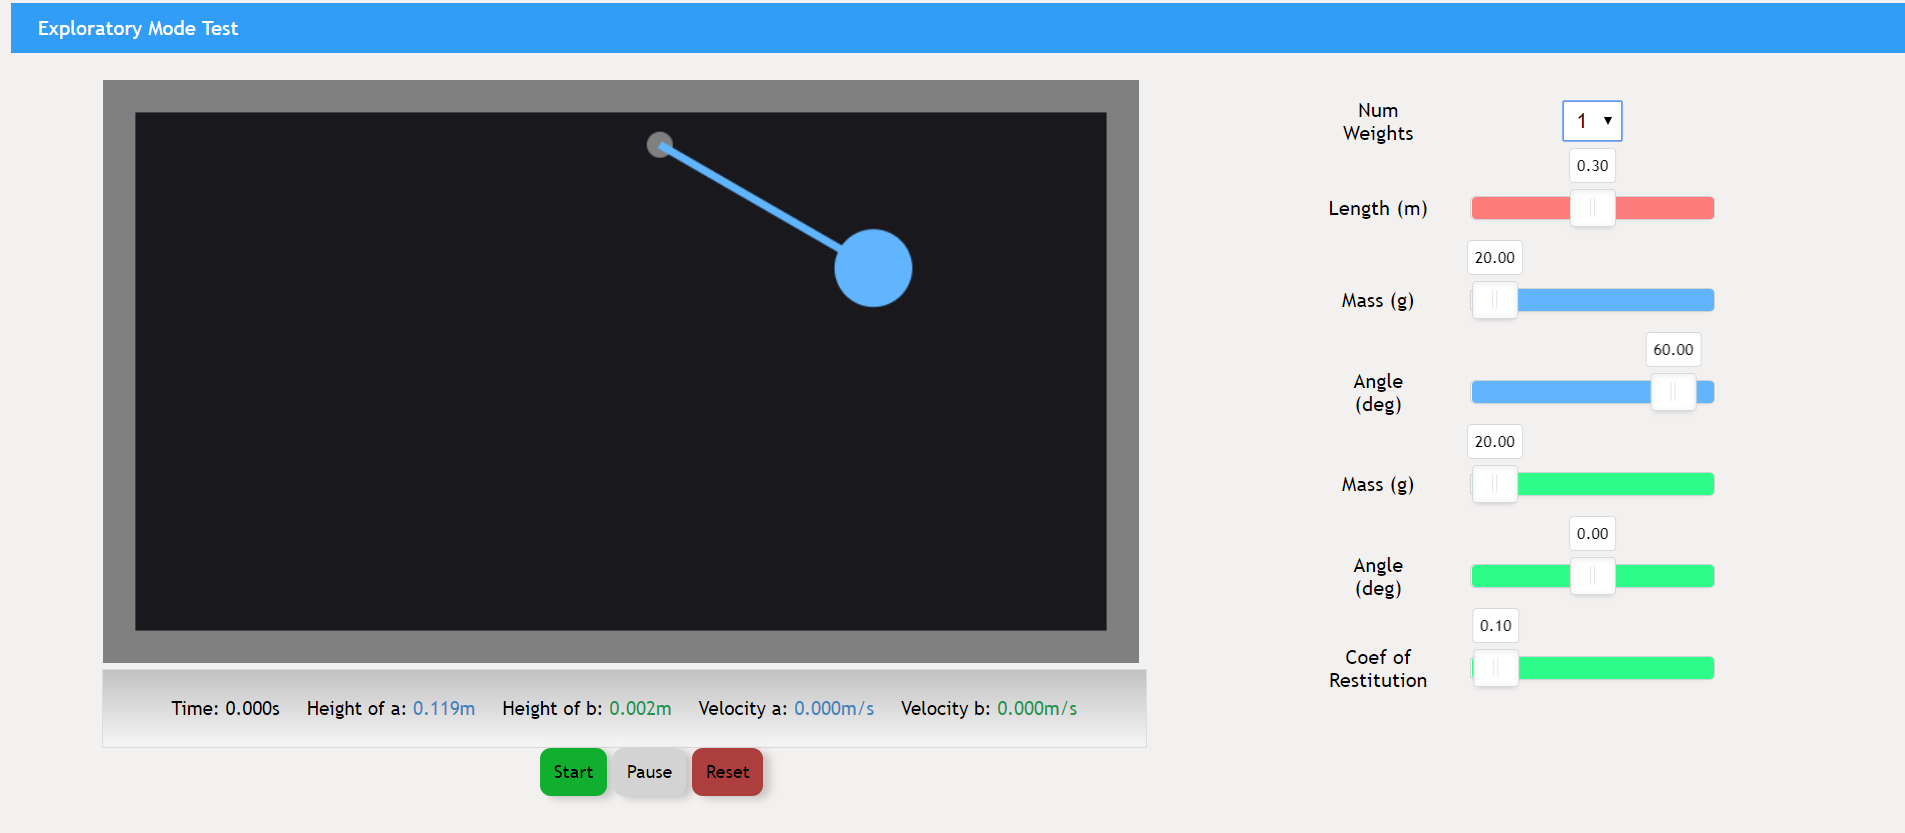
\includegraphics[width=5.5 in]{pictures_beta/exploratory_start_1.png}
  \caption{Exploratory Mode - initial screen}
  \label{fig:Exploratory1}
\end{figure}

\begin{figure}[H]
  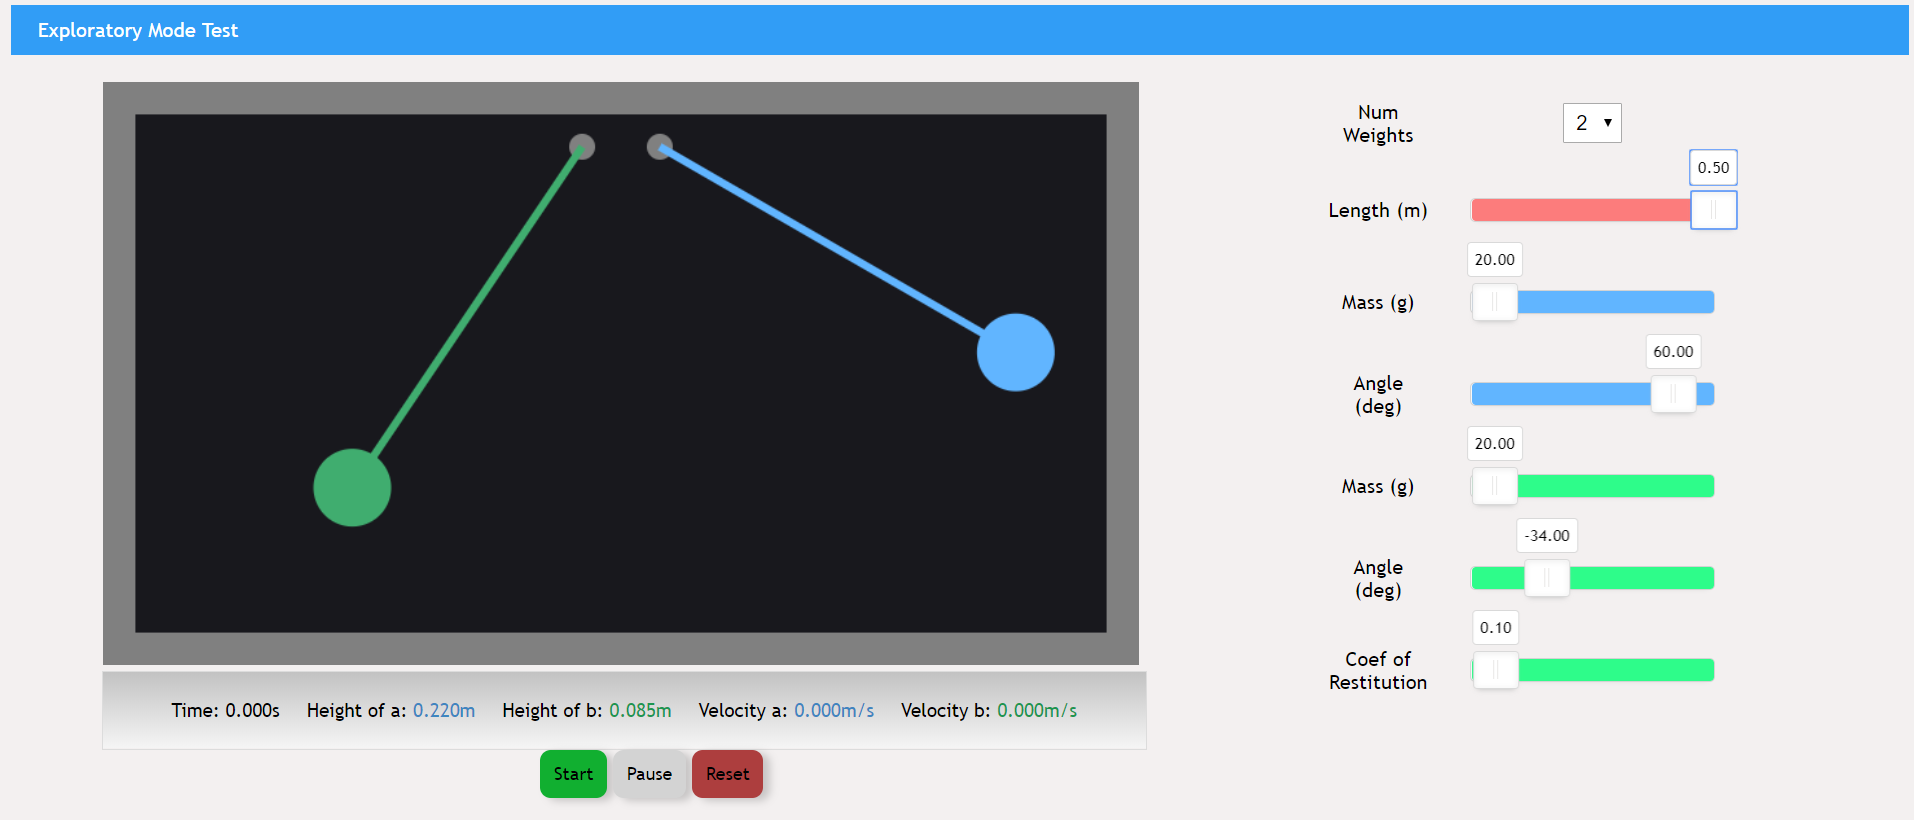
\includegraphics[width=5.5 in]{pictures_beta/exploratory_start_2.png}
  \caption{Exploratory Mode - Two pendulums}
  \label{fig:Exploratory2}
\end{figure}

\begin{figure}[H]
  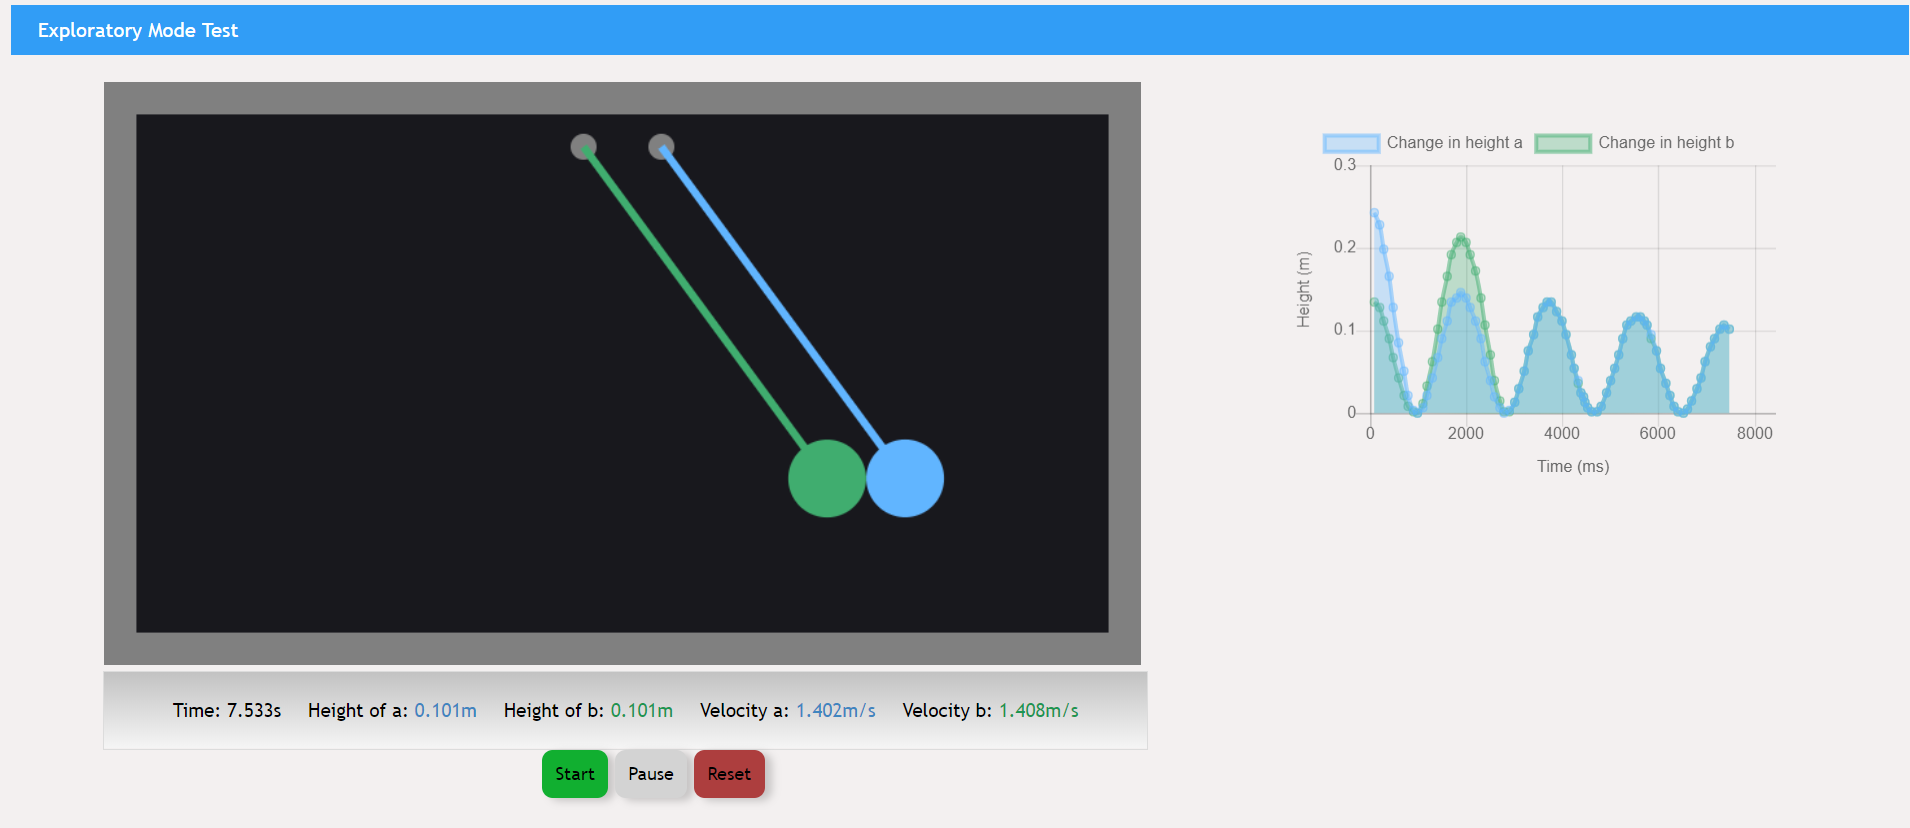
\includegraphics[width=5.5 in]{pictures_beta/exploratory_mid_2.png}
  \caption{Exploratory Mode - Two pendulums while the simulation is running}
  \label{fig:Exploratory2_while}
\end{figure}




\section{Project Implementation}
%show in the document what we have done with pictures and describe it?
\subsection{Cases 1 - 5}

Cases 1-5 all require the features of a simulation, start/reset buttons, live update table, and live update graphs. Each case has different starting conditions for each pendulum - varying the mass, height, and coefficient of restitution (whether the weights stick together or not). Currently, the site is organized that the simulation takes up most of the screen on the left, and the buttons, graph, and table is shown on the right. 

\noindent 
All the animations are made using the physics library Matter.js, and the graphs are made using Chart.js. The animations are constructed by placing each pendulum weight into the world at its appropriate position, attaching a string from the top to the weight, setting its mass and restitution, and letting the physics engine handle the animation. The chart data is linked to the motion of the pendulum. 

\subsection{Exploratory Mode}
Exploratory mode reuses most of the code used in the 5 other cases. The simulation is only changed to use values from the range sliders to the right of the simulation. Whenever the user changes the value of the sliders, the simulation is updated to use those values. After hitting the start button, the live graph is shown to replace the sliders (Shown in Figure\ref{fig:Exploratory2_while}), and the table below the simulation shows live updates of its height and velocity.  

\noindent 
To build the sliders, we used the JavaScript library noUiSlider. It provides functions to easily grab the value from the slider and add features like the tool tip shown above the slider knob. 
The library also has helper callback functions to execute certain functions when an event on the slider is performed. Whenever the slider is moved, the physics engine's inputs change appropriately.

\noindent 
After hooking up the simulation to use the slider values rather than hard-coded values, the physics engine takes care of the rest of the simulation. In Matter.js, objects already have functions in place to set the mass and restitution. Setting the string length and angle involved calculating the pendulum weight's position based on those values, then adding a string from the top to that weight. 

\section{Problems}
\subsection{Libraries}
Some of the JavaScript libraries we initially picked did not work out as we first intended. 
For UI styling, we initially planned on using Bulma.io or Bootstrap, but the libraries did not incorporate well into the website or with the other libraries we planned on using. Efforts were made to try to make the libraries work together, but it seemed more effort than manually coding the layout. To solve this problem, we used flex boxes instead of using those libraries. It took a little more work to manually make a site responsive, but the layout is clean and working fine as of now. 

\subsection{Air resistance}
Another issue we are still trying to handle is the physics engine's inability to mitigate air resistance on a pendulum that should be swinging indefinitely. It is a known issue to the author and the community working on the physics engine; however, no solutions have been merged into the library to solve the issue. The solutions we have come up with to solve this issue so far include adding a slight artificial force to the pendulum to make it go on indefinitely. This works for the first 5 cases. However, in the exploratory case when there are many possible outcomes, this fix will feel finicky. 
\noindent
We may also have to contribute to the open source project and figure out where the error is coming from in Matter.js. After looking at the source code in Matter.js, we found that the simulation velocity/acceleration in the system were decreasing by a factor in the range 0.001 - 0.003 at each time step - depending on the highest point of the pendulum and the pendulum's arm length. When we change this code, for one pendulum the graph looks closer to what we expect as seen in Figure \ref{fig:air_resistance_temp_fix}. However, there is no elegant solution or pattern, that we found so far, to accurately calculate the factor based on the maximum pendulum height. For some cases, this solution can eventually increase the maximum height which is less ideal than the simulation losing energy. For one pendulum, we can have a table of values to match the factor to the maximum angle height. For two pendulums, this solution will not work as well because the path of each of the pendulums is not as predictable. The last solution is to let exploratory mode include a range slider for air resistance, while in the process letting the user know that there will always be air resistance in the simulation. We explained to the client where we are blocked and offered our possible solutions. 

\begin{figure}[!tbp]
  \centering
  \begin{minipage}[b]{0.4\textwidth}
      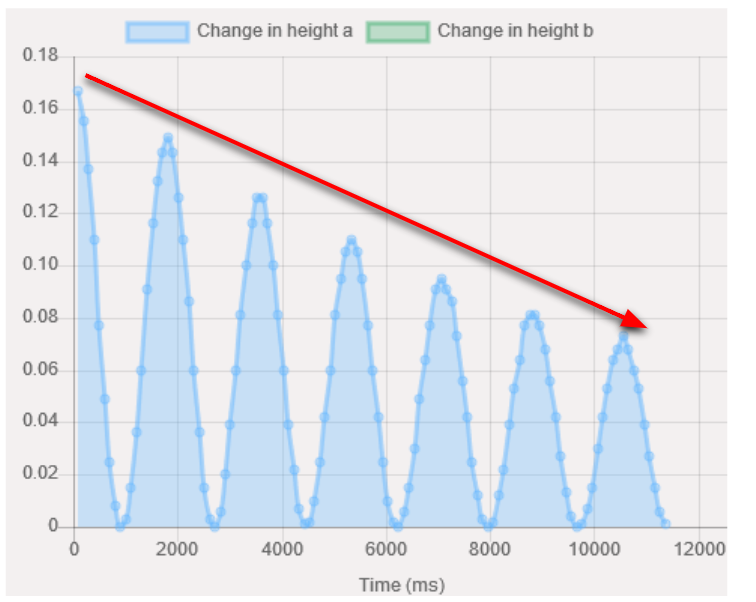
\includegraphics[width=\textwidth]{pictures_beta/damping_arrow.png}
      \caption{Graph in exploratory mode with damping}
      \label{fig:air_resistance1}
  \end{minipage}
  \hfill
  \begin{minipage}[b]{0.4\textwidth}
      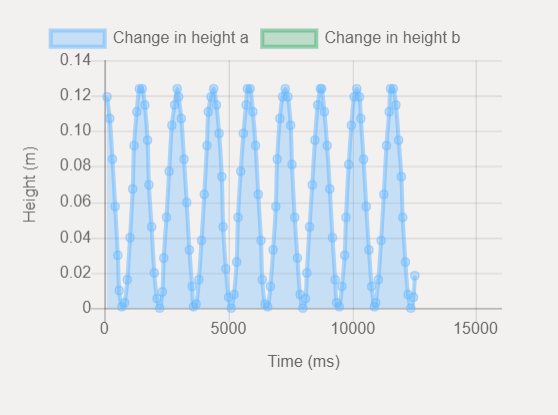
\includegraphics[width=\textwidth]{pictures_beta/air_resistance_fix.png}
      \caption{Exploratory graph - fix for one pendulum}
      \label{fig:air_resistance_temp_fix}
  \end{minipage}
\end{figure}

\noindent
Also the values in the graph might not be entirely accurate in a perfect pendulum system since the graph receives values directly from the simulation, and we had to apply a slight artificial force to get the pendulum to an accurate position. The end values are accurate - which is the main focus of the exercise; however, on closer inspection of the graph, the values at certain times might be different to the real physical system.  To solve the graph values, we can calculate the values separately from the animation and sync it properly with the animation.

\section{What is Left}
We still need to work out some small bugs that have been introduced throughout the development of the project, as well as minor features which we are missing. In exploratory mode, We need to add a set of radio buttons, that control what data is displayed on the graph. The user can pick among a velocity, acceleration, or height graph. The website can also have a help/info button or tool tips when the user hovers over an item. Also, in exploratory mode, some of the calculations for velocity and height are off by a small amount, and sometimes do not match what is happening in the simulation. We will also continue to work on the air resistance problem. 

%There has also been stylistic choices pointed out by the client that need to be modified before the beta due date. In all the cases, we need to make the string not appear over the weight. One solution we plan to implement is to change the color of the string to the color of the weight. The size of the weight, and the size and position of the anchor point, are still up to debate. Finally, the position of the feedback data and the control buttons may be changed to be below the simulation.

\noindent 
There are stretch goals that were put in place at the start of the capstone project between the client and us that is still possible to get started on next term. This stretch goal is to create five additional simulations based on interactions with a spool along with its own separate exploratory mode. Everything we have learned from our current set of simulations should allow us to create a new set, even if the new simulations are different in function.

\end{document}

